\section{Exploratory Data Analysis}
\label{sec:eda}

In this section we focus on the two benchmarks WTI and Brent, since "returns" are only a meaningful concept
for a traded price series, not for a level/flow series such as OPEC spare capacity.

\subsection{Distributional Plots}

\begin{figure}[H]
  \centering
  \begin{subfigure}[b]{0.48\textwidth}
    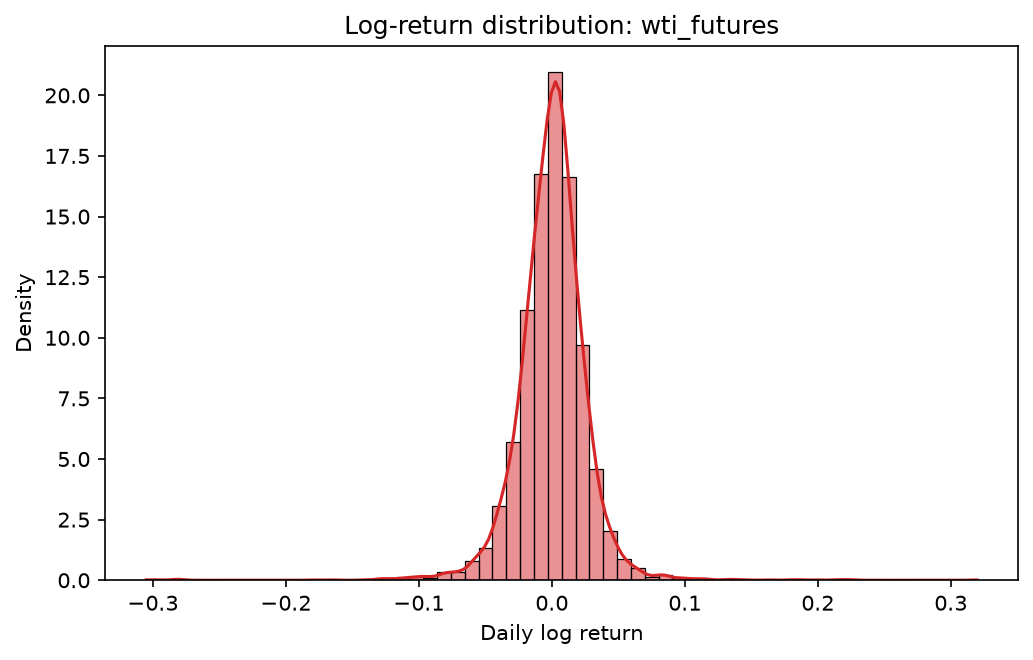
\includegraphics[width=\textwidth]{figures/return_dist_wti_futures.png}
    \caption{WTI daily log-return distribution}
  \end{subfigure}
  \hfill
  \begin{subfigure}[b]{0.48\textwidth}
    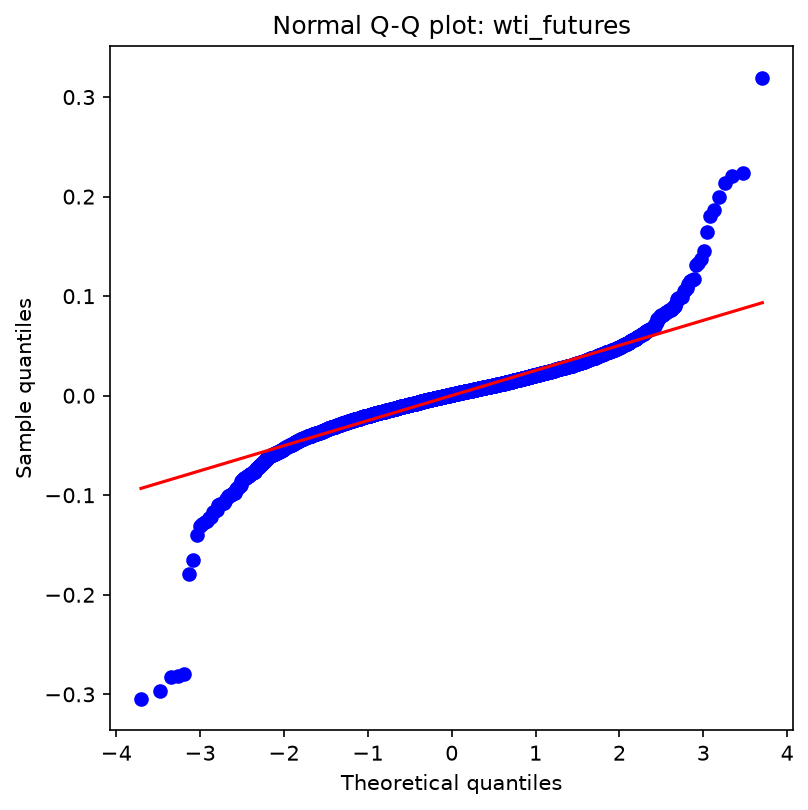
\includegraphics[width=\textwidth]{figures/qq_wti_futures.png}
    \caption{WTI daily log-return Q-Q plot}
  \end{subfigure}
  \caption{Distributional diagnostics for WTI daily log returns.}
  \label{fig:wti-distribution}
\end{figure}

\subsection{Time Series Plots}

\begin{figure}[H]
  \centering
  \begin{subfigure}[b]{0.48\textwidth}
    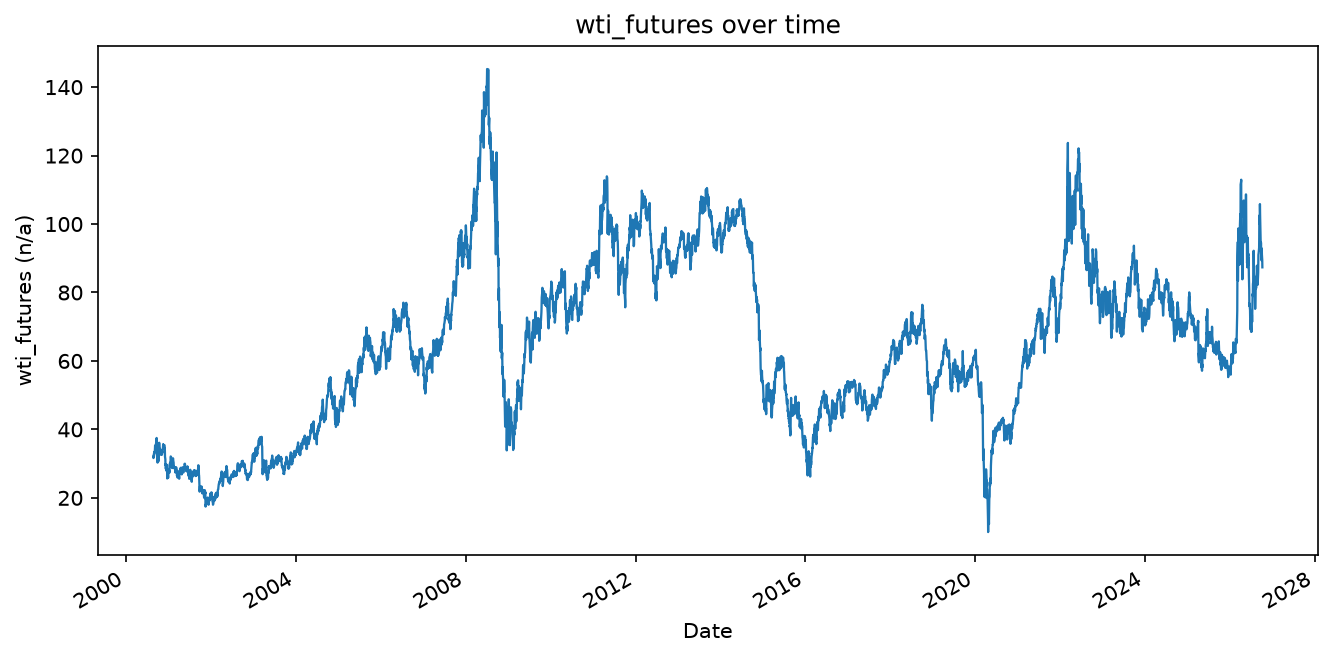
\includegraphics[width=\textwidth]{figures/level_deep_wti_futures.png}
    \caption{WTI price level}
  \end{subfigure}
  \hfill
  \begin{subfigure}[b]{0.48\textwidth}
    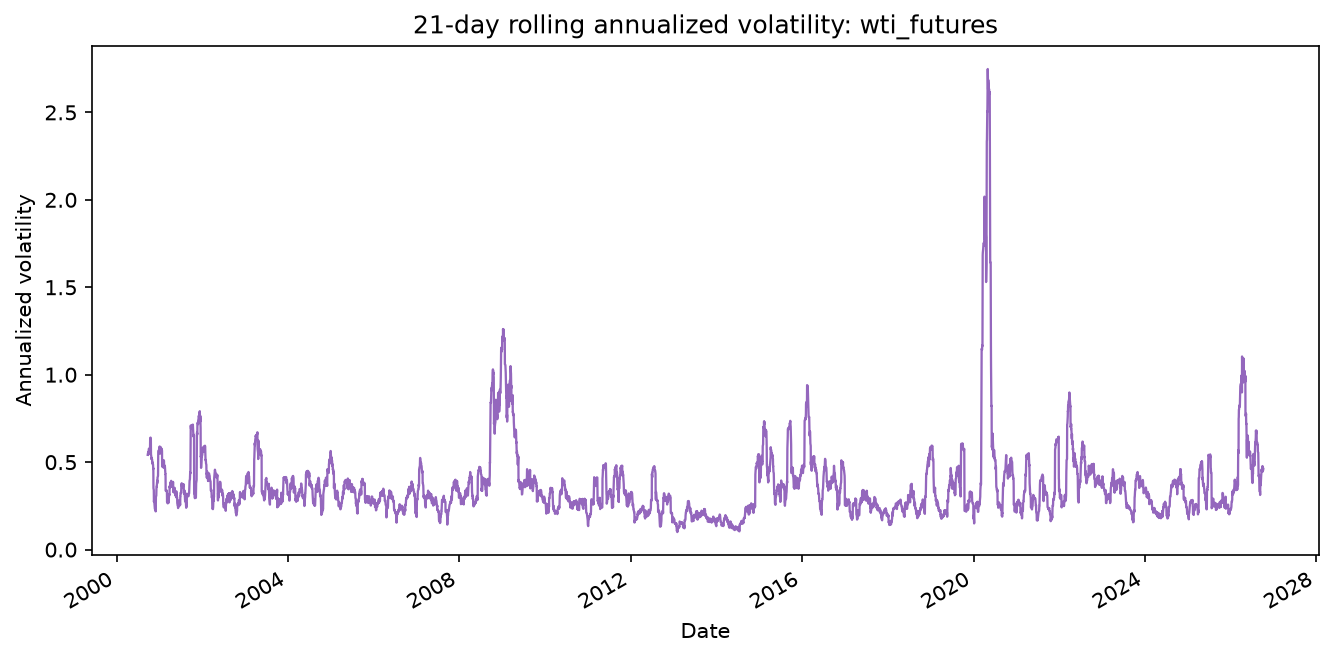
\includegraphics[width=\textwidth]{figures/vol_wti_futures.png}
    \caption{21-day rolling annualised volatility}
  \end{subfigure}
  \caption{WTI price level and rolling volatility, full sample.}
  \label{fig:wti-timeseries}
\end{figure}

\begin{figure}[H]
  \centering
  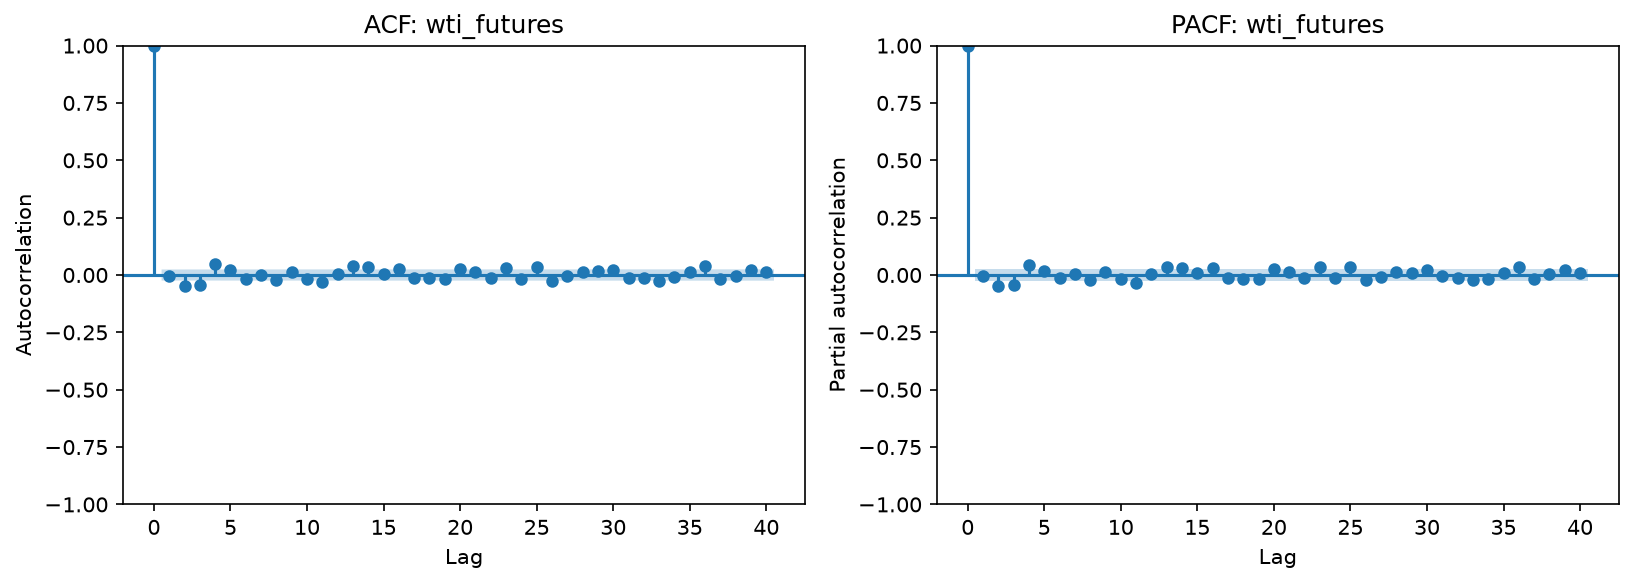
\includegraphics[width=0.85\textwidth]{figures/acf_wti_futures.png}
  \caption{ACF and PACF of WTI daily log returns (40 lags).}
  \label{fig:wti-acf}
\end{figure}

\subsection{Multivariate Plots}

\begin{figure}[H]
  \centering
  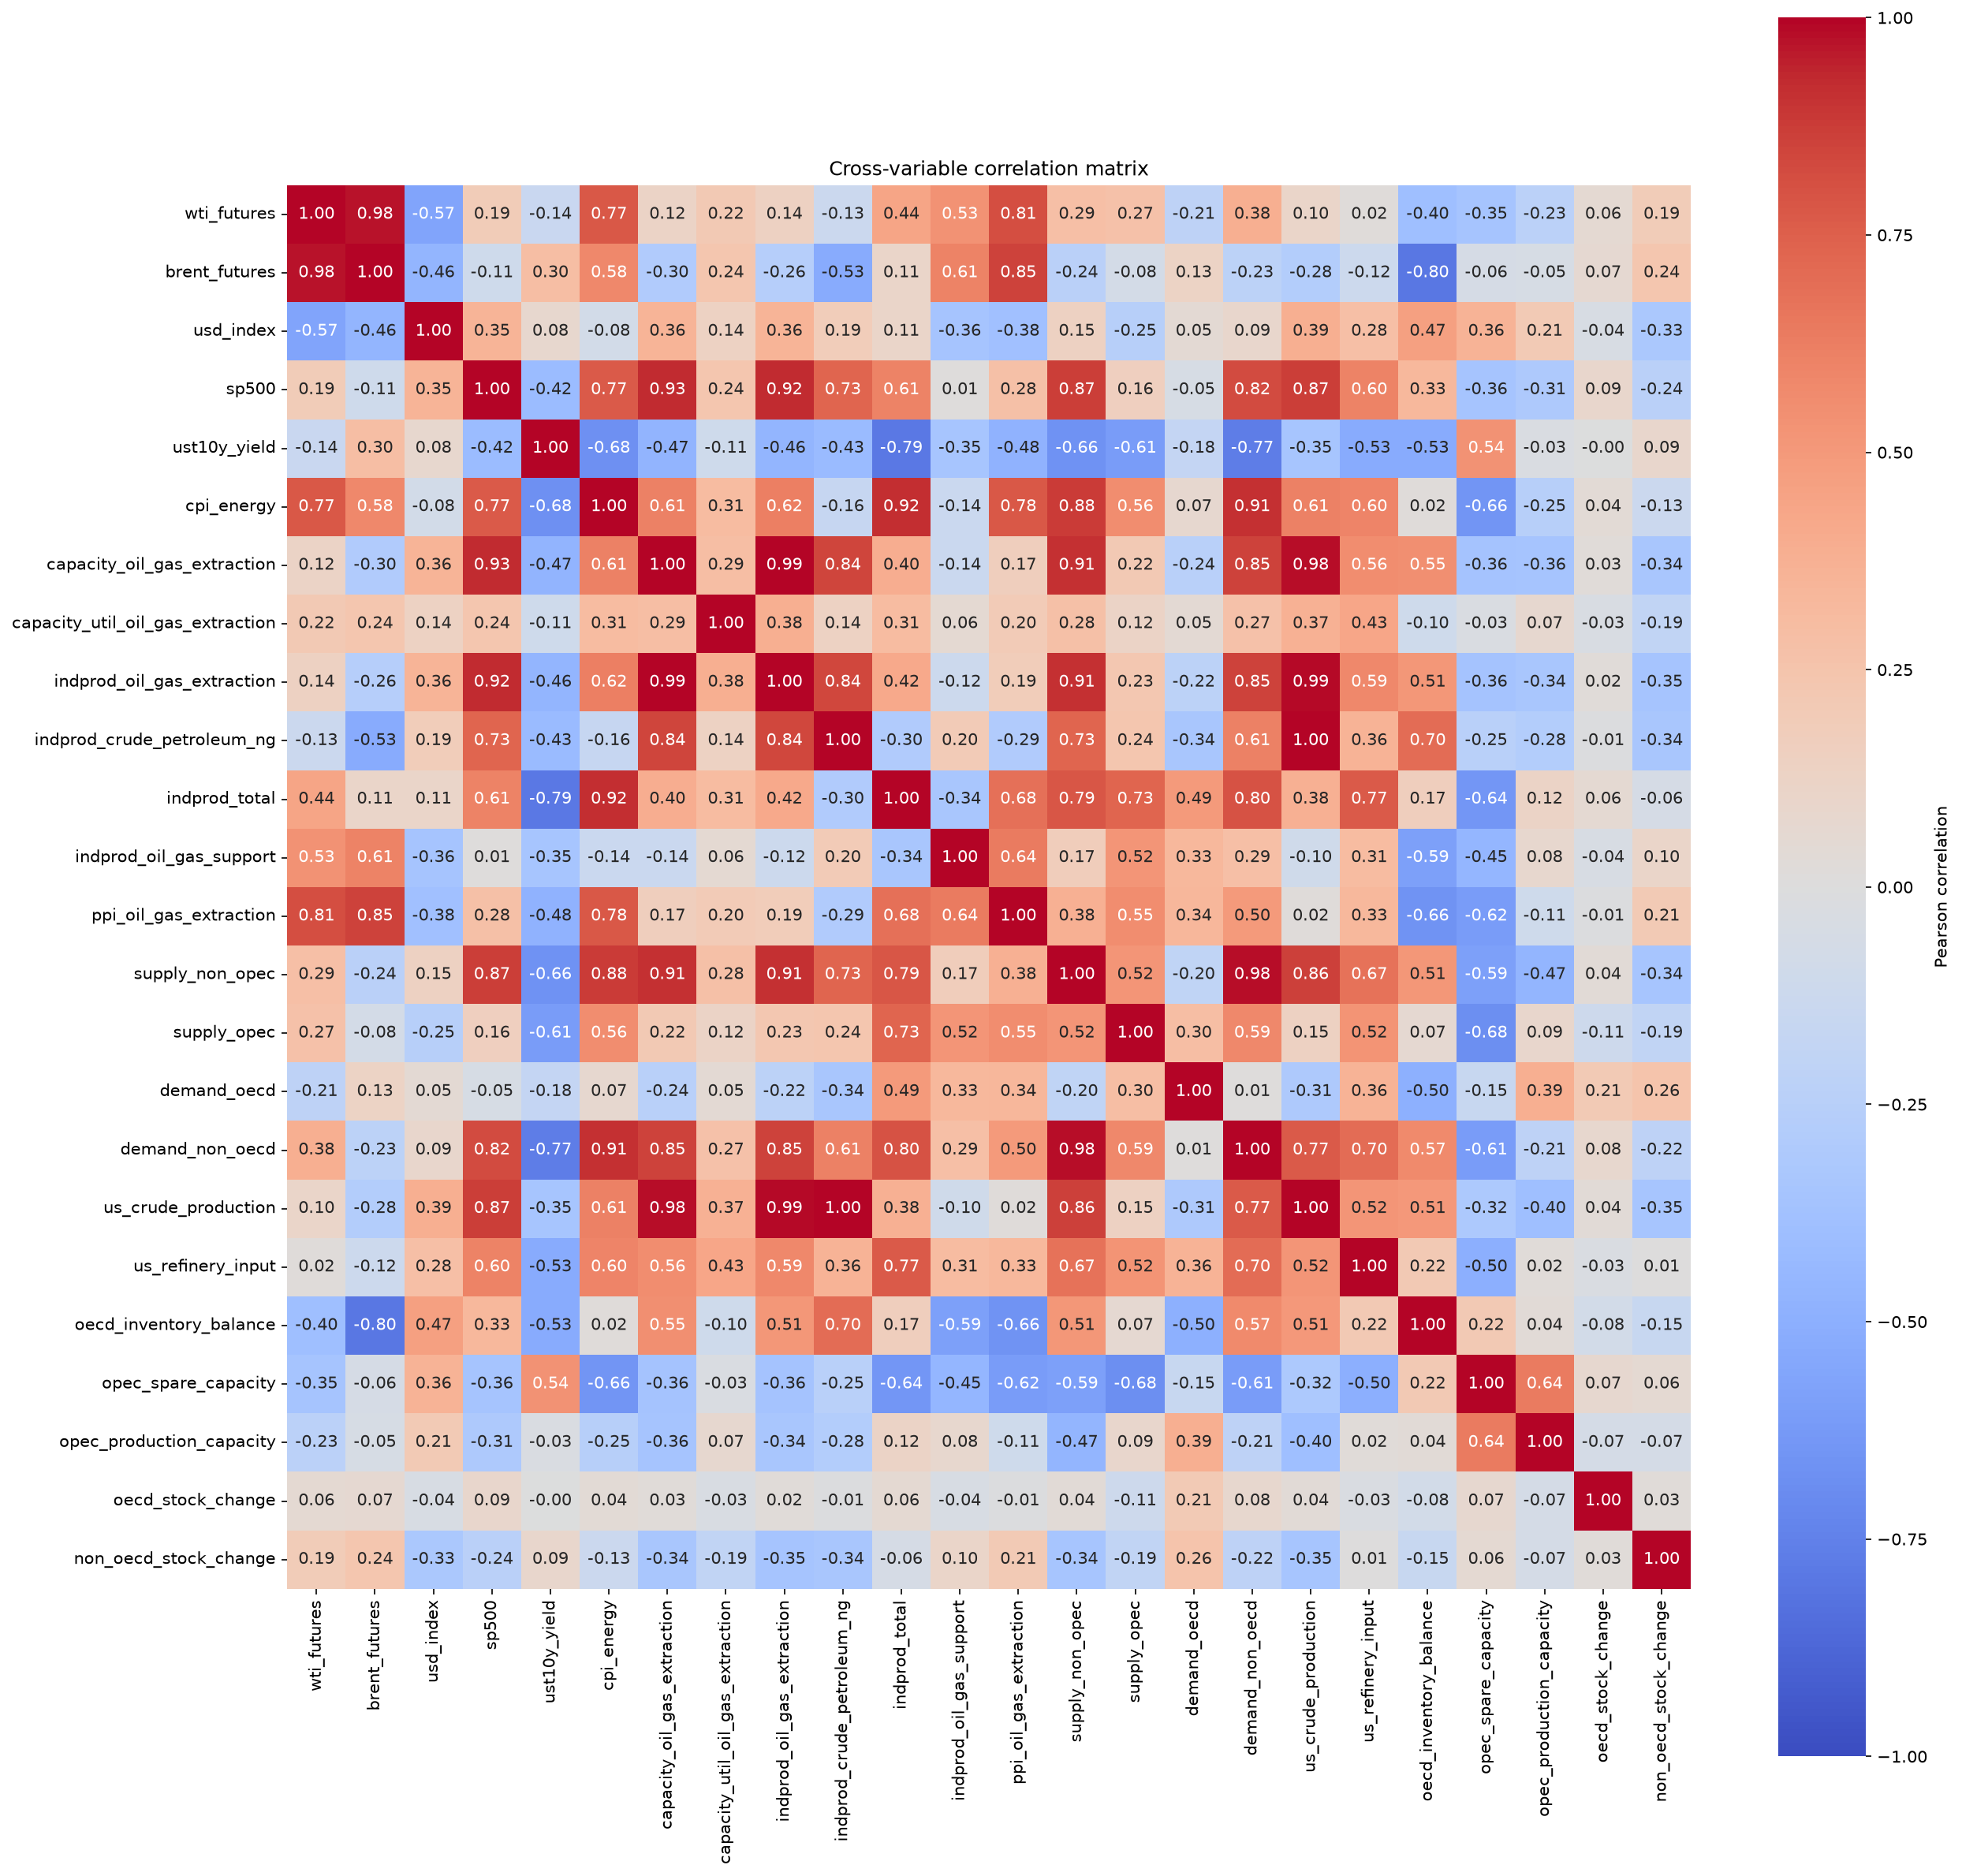
\includegraphics[width=\textwidth]{figures/correlation_heatmap_all.png}
  \caption{Pearson correlation matrix across all 24 monthly-aligned series.}
  \label{fig:correlation-heatmap}
\end{figure}

\begin{figure}[H]
  \centering
  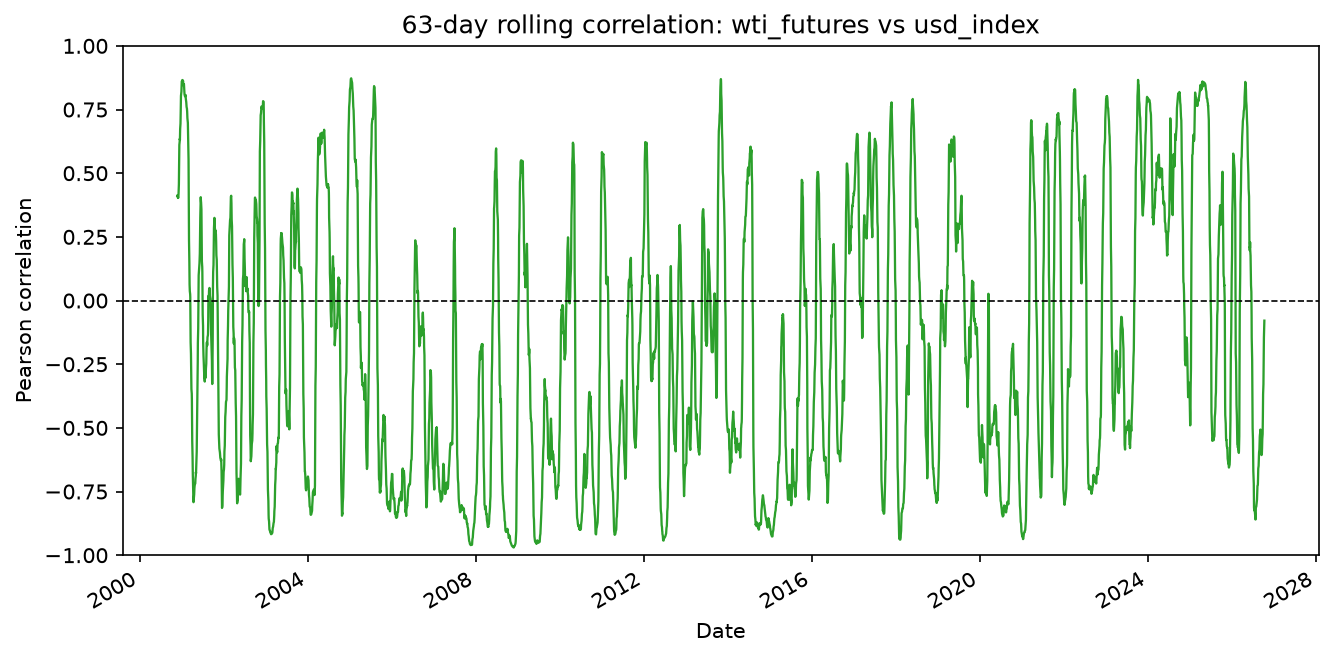
\includegraphics[width=0.85\textwidth]{figures/rolling_corr_wti_usd.png}
  \caption{63-day rolling correlation, WTI futures vs.\ the US dollar index.}
  \label{fig:rolling-corr}
\end{figure}

\begin{figure}[H]
  \centering
  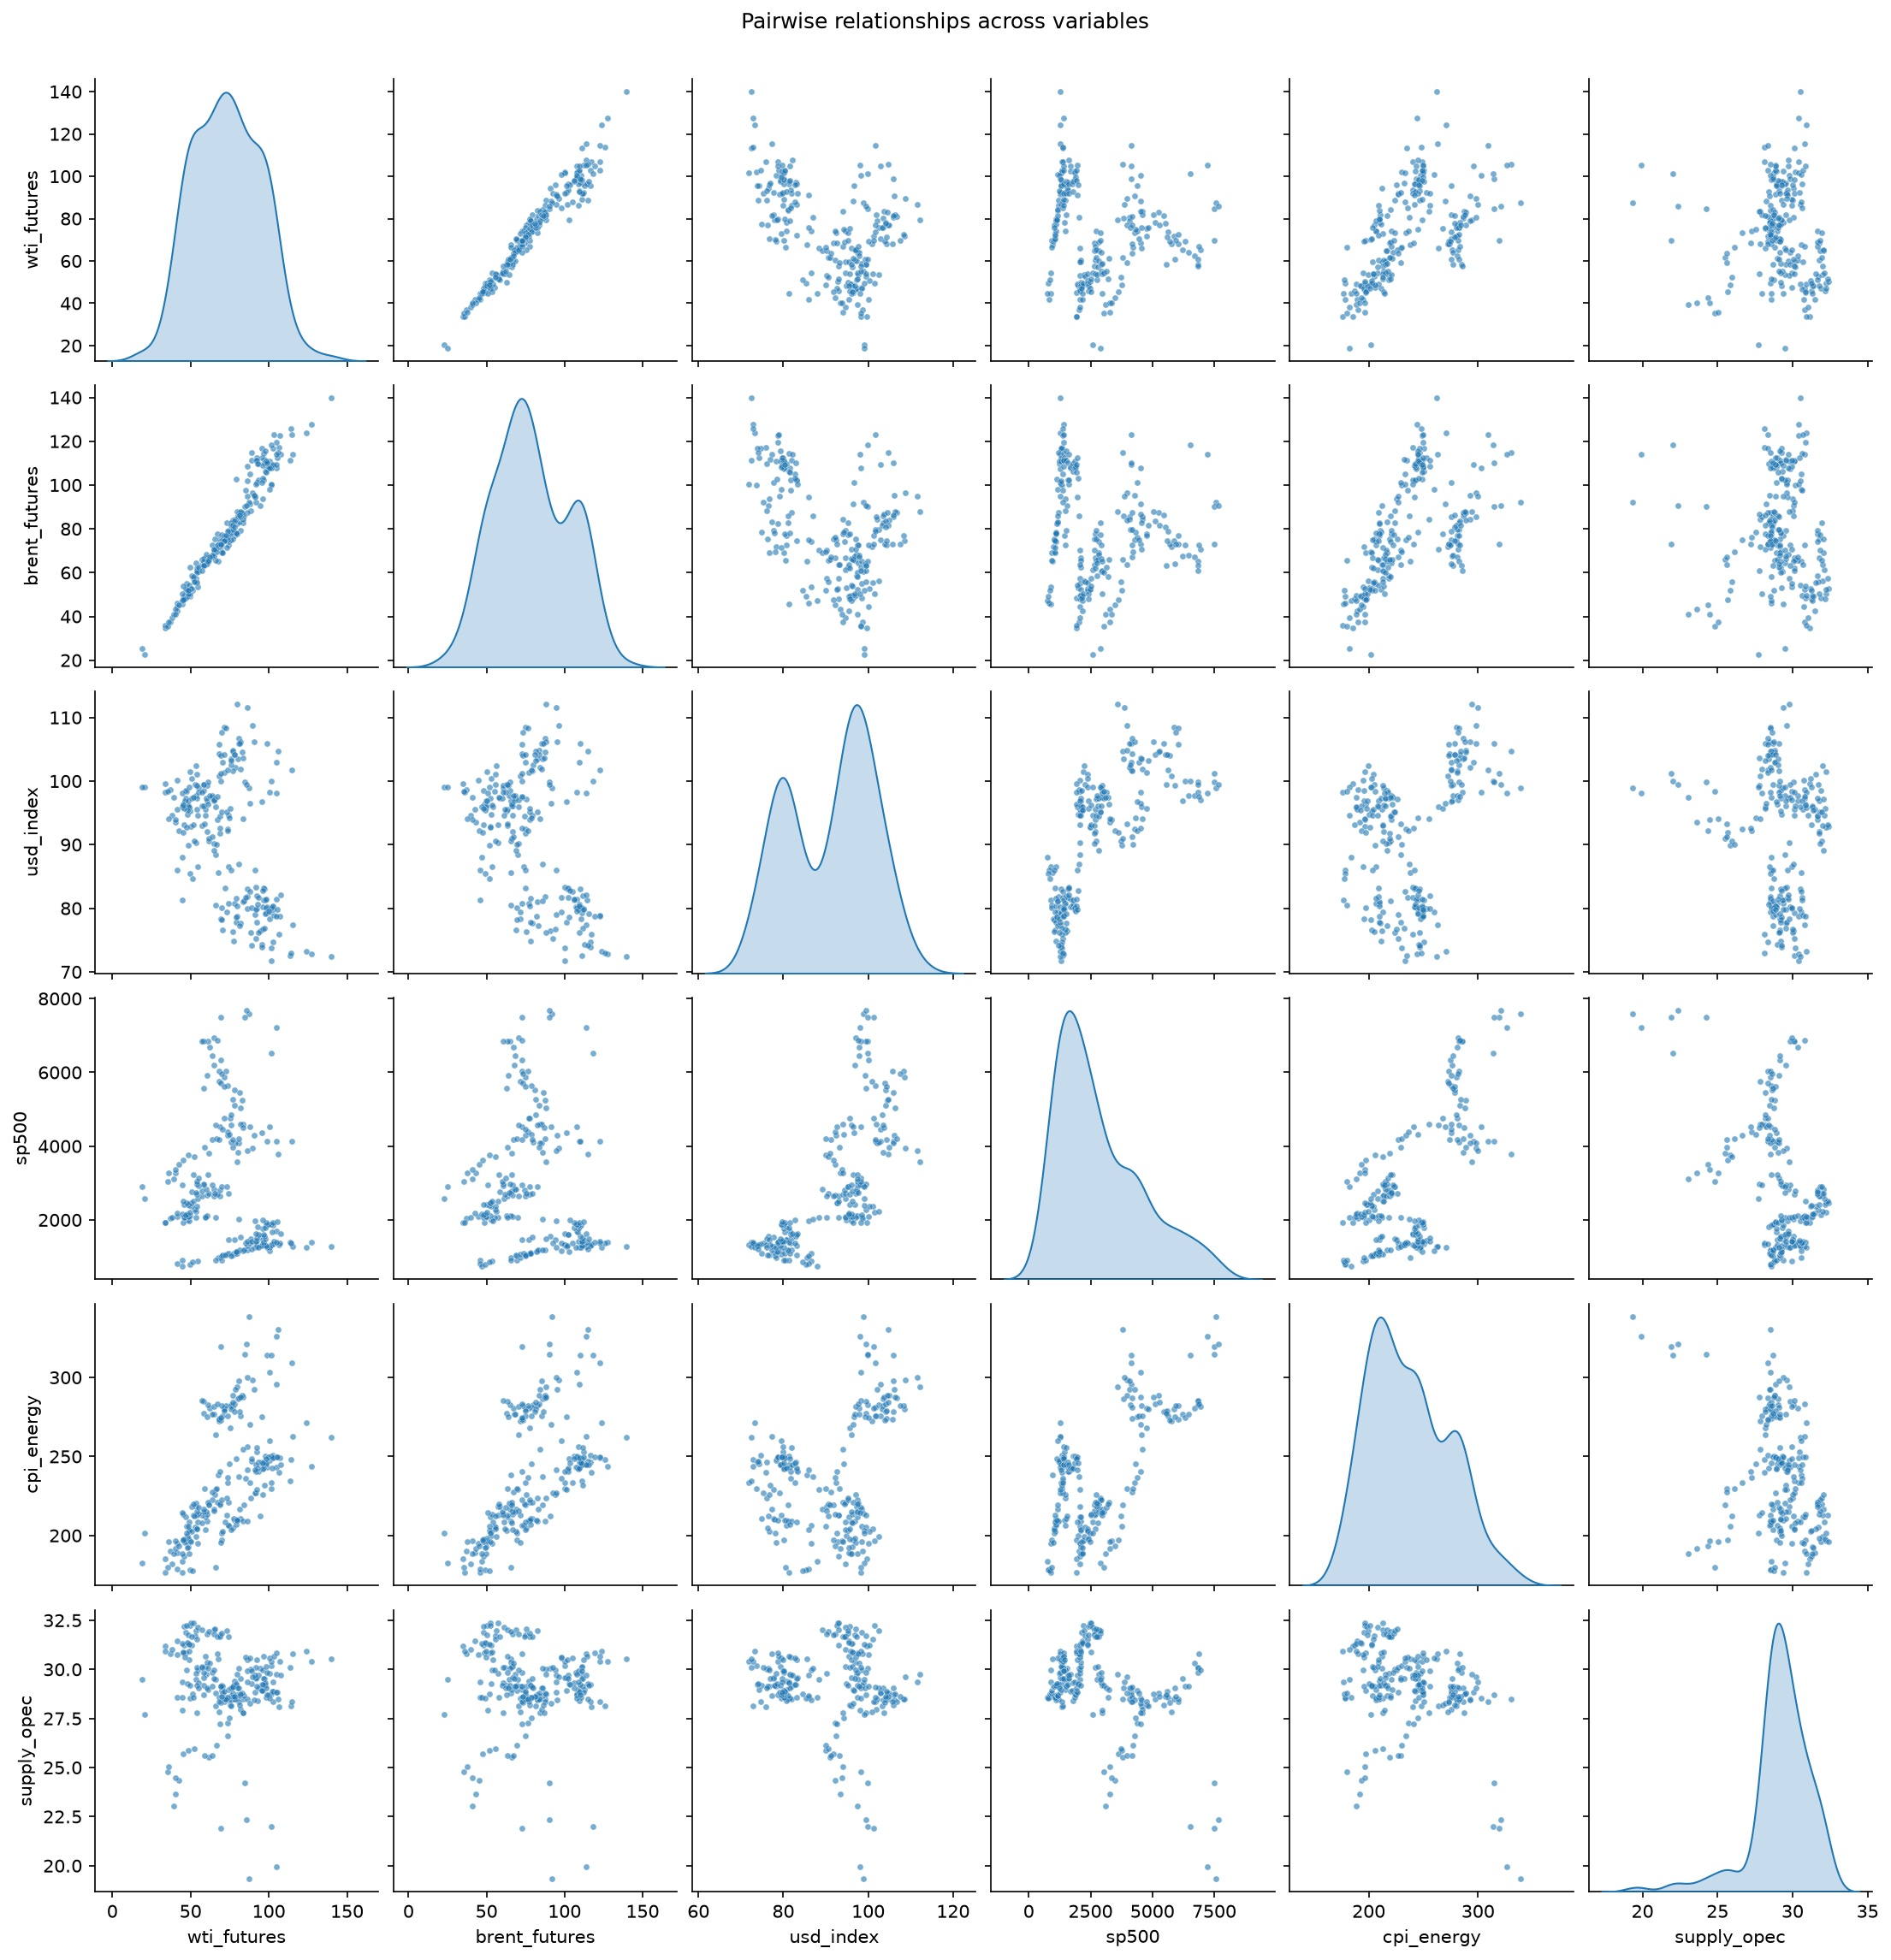
\includegraphics[width=\textwidth]{figures/scatter_matrix_headline.png}
  \caption{Scatter matrix of a curated headline subset (both crude
    benchmarks, the US dollar index, the S\&P 500, the energy CPI index, and
    OPEC supply), resampled to month-end.}
  \label{fig:scatter-matrix}
\end{figure}

\section{Stylized Facts}
\label{sec:stylized-facts}

Here we use statistics computed on daily log returns (see Table~\ref{tab:stylized-facts}) for the two crude benchmarks and the above figures for our analysis.

\begin{table}[h]
  \centering
  \caption{Stylized-facts statistics on daily log returns.}
  \label{tab:stylized-facts}
  \begin{tabular}{lrr}
    \toprule
     & WTI & Brent \\
    \midrule
    Observations & 6{,}557 & 4{,}775 \\
    Annualised mean return & 3.87\% & 1.39\% \\
    Annualised volatility & 42.6\% & 38.7\% \\
    Skewness & $-0.51$ & $-0.77$ \\
    Excess kurtosis & 18.74 & 11.63 \\
    Jarque-Bera statistic & 96{,}264 & 27{,}389 \\
    Jarque-Bera $p$-value & $<0.001$ & $<0.001$ \\
    ACF of returns, lag 1 & $-0.004$ & $-0.018$ \\
    ACF of squared returns, lag 1 & 0.46 & 0.20 \\
    ACF of squared returns, lag 5 & 0.25 & 0.12 \\
    \bottomrule
  \end{tabular}
\end{table}

\textbf{(a)}
The level plots (Figure~\ref{fig:wti-timeseries}) show oil behaving less like
a smoothly-trending equity index and more like a regime-switching series:
multi-year bull/bear swings (the 2000-08 rally, the 2008-09 collapse, the
2014-16 collapse, the 2020 COVID crash, and the 2022 spike) punctuated by
sharp, short-lived shocks. The rolling-volatility plot shows that volatility
itself is clustered and regime-dependent, with calm multi-year stretches
interrupted by violent spikes exceeding 2.5$\times$ the typical annualised
level in April 2020. That episode is itself a uniquely oil-specific
phenomenon: as discussed in Section~\ref{sec:data-cleaning}, WTI's
near-month contract briefly traded at a negative price on 20 April
2020 — essentially impossible for an equity or FX price, but a direct
consequence of physical-delivery settlement when storage capacity is
exhausted. Our general-purpose cleaning pipeline treats that single
observation as bad data and imputes it away, which is a transparent,
documented trade-off rather than a silent one, and the event itself remains
a genuine, worth-noting stylized fact about oil specifically.

\textbf{(b)} WTI returns show mild negative skewness ($-0.51$, i.e.\ large
down-moves are somewhat more extreme than large up-moves) and strongly
leptokurtic, fat-tailed behaviour (excess kurtosis of 18.74 against 0 for a
Normal distribution); Brent shows the same pattern (skewness $-0.77$, excess
kurtosis 11.63). The Jarque-Bera test rejects normality overwhelmingly for
both series ($p < 0.001$), consistent with the pronounced bowing away from
the theoretical line visible in the Q-Q plot (Figure~\ref{fig:wti-distribution})
beyond roughly $\pm 2$ standard deviations.

\textbf{(c)} Essentially none at the level of raw returns: the lag-1 autocorrelation is $-0.004$
(WTI) and $-0.018$ (Brent), and the ACF/PACF plot
(Figure~\ref{fig:wti-acf}) shows no economically significant spikes beyond
lag 0 — consistent with (weak-form) market efficiency, i.e.\ the sign of
tomorrow's return is not linearly predictable from today's. The squared returns, however, tell a very different story: lag-1 autocorrelation of squared returns is 0.46 (WTI) and 0.20 (Brent), still 0.25/0.12 at lag 5 — a strong, slowly-decaying autocorrelation. This is the
textbook signature of volatility clustering: returns themselves are unpredictable, but the magnitude of returns is highly persistent, motivating a regime-switching (Hidden Markov Model) approach.

\textbf{(d)} 
\begin{itemize}
	\item  A
	negative, but highly unstable, correlation with the US dollar index: the full-sample level correlation is $-0.57$ (WTI) / $-0.46$ (Brent) (Figure~\ref{fig:correlation-heatmap}), yet the 63-day rolling correlation (Figure~\ref{fig:rolling-corr}) oscillates repeatedly between roughly $-1$
	and $+1$ across the whole sample with no single stable regime — the textbook "stronger dollar, cheaper oil" relationship holds on average but is far too unstable to use as a reliable short-horizon hedge on its own.
	\item WTI and Brent correlate at 0.98 in levels and track each other almost one-for-one, as expected for two prices of the same underlying global commodity linked by arbitrage.
	\item Oil correlates positively, but only
	moderately, with broad inflation/risk-sentiment variables — the energy CPI
	index (0.77 WTI, 0.58 Brent) more so than the S\&P 500 (0.19 WTI, $-0.11$
	Brent) — i.e.\ energy prices are a meaningful component of realised
	inflation, not merely a passive responder to broad equity risk sentiment.
	\item Geopolitical/supply variables correlate only weakly and inconsistently
	with price (e.g.\ OPEC supply: 0.27 WTI / $-0.08$ Brent; non-OPEC supply:
	0.29 WTI / $-0.24$ Brent) — far weaker than the financial variables above —
	consistent with our central thesis (Section~\ref{sec:problem-formulation})
	that oil-price dynamics are better captured by a non-linear, graphical/probabilistic model of many interacting physical and financial drivers than by simple pairwise linear correlation.
\end{itemize}